\section{Analyse descendante}
    \begin{figure}[h] 
        \centering      
        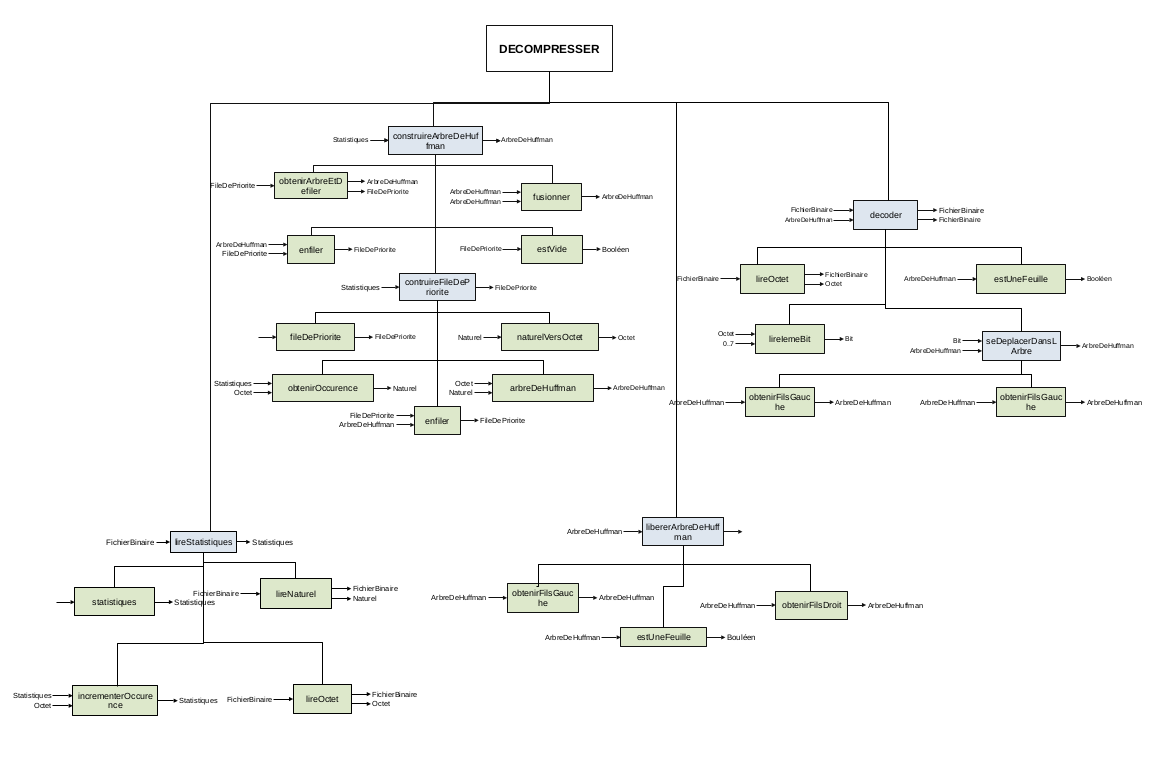
\includegraphics[width=1.1\textwidth]{decompresser.png}
        \caption{Analyse descendante de la décompression}
        \label{fig:exemple}
    \end{figure}
    
\newpage
\section{Conception Préliminaire}
    \begin{algorithme}
    \signatureFonction{lireStatistiques}{fb : \fichierbinaire}{\statistiques}{estOuvert(fb) et (mode(fb) $=$ lecture)}
\end{algorithme}
    \begin{algorithme}
    \signatureFonction{construireFileDePriorite}{s : \statistiques}{\filedepriorite}{}
\end{algorithme}
    \begin{algorithme}
    \signatureFonction{construireArbreDeHufmman}{s : \statistiques}{\arbredehuffman}{}
\end{algorithme}
    \begin{algorithme}
    \signatureProcedure{seDeplacerDansLArbre}
{\paramEntree{bit : \bit, a1 : \arbredehuffman}, \paramSortie{a2 : \arbredehuffman}}{}
\end{algorithme}
    \begin{algorithme}
    \signatureProcedure{decoder}
{\paramEntree{a : \arbredehuffman, longueur : \naturel}, \paramEntreeSortie{fb1 : \fichierbinaire, fb2 : \fichierbinaire}}{estOuvert(fb1) et (mode(fb1) $=$ lecture) et estOuvert(fb2) et (mode(fb2) $=$ écriture)}
\end{algorithme}
    \begin{algorithme}
    \signatureProcedure{decompresser}{\paramEntreeSortie{fCompresse : \fichierbinaire}, \paramSortie{fDecompresse : \fichierbinaire}}{}
\end{algorithme}

\newpage
\section{Conception Détaillée}
    \begin{algorithme}
    \fonction{lireStatistiques}{fb : \fichierbinaire}{\statistiques}{estOuvert(fb) et (mode(fb) $=$ lecture)}
    {n, i : \naturel , s : \statistiques}
    {
    	\affecter{s}{statistiques()}
    	\commentaire{La fonction lireStatistiques est utilisée quand le curseur est au bon endroit et l'on peut donc directement lire les statistiques qui sont des naturels}
    	\pour{i}{0}{255}{}
    	{
    		\instruction{lireNaturel(fb, n)}
        	\affecter{s[i]}{n}
    	}
    \retourner{s}
    }
\end{algorithme}
    \begin{algorithme}
    \fonction{construireFileDePriorite}{s : \statistiques}{\filedepriorite}{}
    {fdp : \filedepriorite, octet : \octet, occurence : \naturel}
    {
        \affecter{fdp}{fileDePriorite()}
        \pour{o}{ 0}{255}{}
        {
            \affecter{octet}{naturelVersOctet(o)}
            \affecter{occurence}{obtenirOccurence(s, octet)}
            \sialors{occurence > 0}{
                \instruction{enfiler(fdp, arbreDeHuffman(octet, occurence))}
            }
        }
        \retourner{fdp}
    }
\end{algorithme}
    \begin{algorithme}
	\fonction{construireArbreDeHuffman}{s : \statistiques}{\arbredehuffman}{}
	{fdp : \filedepriorite, dernierElement : \booleen, a1, a2, aFusion : \arbredehuffman}
    {
    	\affecter{fdp}{construireFileDePriorite(s)}
    	\affecter{dernierElement}{estVide(fdp)}
    	\tantque{non(dernierElement)}
    	{
    		\instruction{obtenirElementEtDefiler(fdp, a1)}
    		\sialorssinon{estVide(fdp)}
    		{
    			\affecter{dernierElement}{VRAI}
    		}
    		{
    			\instruction{obtenirElementEtDefiler(fdp, a2)}
    			\affecter{aFusion}{fusionner(a1, a2)}
    			\instruction{enfiler(fdp, aFusion)}
    		}
    	}
    	}
    	\retourner{a1}
    }
\end{algorithme}
    \begin{algorithme}
    \procedure{seDeplacerDansLArbre}{\paramEntree{bit : bit}, \paramEntreeSortie{arbreCourant : ArbreDeHuffman}}{}{}
    {
        \sialors{bit = 0}
        {
            \affecter{arbreCourant}{obtenirFilsGauche(arbreCourant)}
        }
        \sialors{bit = 1}
        {
            \affecter{arbreCourant}{obtenirFilsDroit(arbreCourant)}
        }
    }
\end{algorithme}

    \begin{algorithme}
    \procedure{decoder}{\paramEntree{aHuff : \arbredehuffman, longueur : \naturel}, \paramEntreeSortie{fb1:\fichierbinaire, fb2 : \fichierbinaire}}{}{compteurOctetsDecodes : \naturel}
    {
       \affecter{aTemp}{aHuff}
       \affecter{compteurOctetsDecodes}{0}
       \tantque{compteurOctetsDecodes <= longueur}{
       		\affecter{OctetCourant}{lireOctet(fb1)}
       		\pour{i}{0}{7}{}
       		{
       			\affecter{Bit}{IemeBit(OctetCourant,i)}
       			\instruction{seDeplacerDansLArbre(bit,atemp)}
       			\sialors{estUneFeuille(atemp)}{
       				\affecter{octetDecodé}{obtenirOctet(aTemp)}
       				\instruction{écrireOctet(octetDecodé, fb2)}
       				\affecter{compteurOctetsDecodes}{compteurOctetsDecodes+1}
       				\affecter{aTemp}{aHuff}
       				}
       			}
       		}
    }
    
\end{algorithme}
    \begin{algorithme}
	\procedure{decompresser}{\paramEntreeSortie{fCompresse : \fichierbinaire}, \paramSortie{fDecompresse : \fichierbinaire}}
	{estOuvert(fCompresse) et (mode(fCompresse) $=$ lecture)}
	{i, id, longueur : \naturel, s : \statistiques, abh : \arbredehuffman, octetUnique : \octet}
    {
		\instruction{positionnerAuDebut(fCompresse)}
		\instruction{ouvrir(fDecompresse, ecriture)}
    	\instruction{lireNaturel(fCompresser, id)}
		\\
    	\commentaire{On vérifie si on retrouve bien notre identifiant (ici 1000 sous sa forme de naturel), si ce n'est pas le cas, on n'a pas a décompresser le fichier}
    	\sialors{id = 1000}{   
			\instruction{lireNaturel(fCompresser, longueur)}
			\\\commentaire{Cas particulier d'un fichier vide}
			\sialors{(longueur > 0)}{
				\instruction{lireStatistiques(fCompresser, s)}
				\instruction{construireArbreDeHuffman(s, abh)}
				\\\commentaire{Cas particulier d'un fichier contenant un seul octet (présent plusieurs fois ou non)}
				\sialorssinon{estUneFeuille(abh)}
				{
					\affecter{octetUnique}{octetVersNaturel(obtenirOctet(abh))}
					\pour{i}{1}{longueur}{}{
						\instruction{ecrireOctet(fDecompresse, octetUnique)}
					}
				}
				{
					\instruction{decoder(abh, longueur, fCompresse, fDecompresse)}
				}
				\instruction{liberer(abh)}
			}
    	}
		\instruction{fermer(fDecompresse)}
    }
\end{algorithme}